\begin{enumerate}
	\item Go to \url{https://cocalc.com/} in a web browser.
	\item At the top right of the screen, click on the ``Sign Up''
		link.
	\item You'll need to check the box that says ``I agree to the Terms of Service.''  There is also a ``Privacy Policy'' that is included by reference into the Terms of Service.
	\item It also asks you to select the software that you plan to use.  At a minimum select ``SageMath.''  There's also an ``Everything!'' option if you feel adventurous.
	\item Next you'll be asked for your email address, your name, and to choose a password -- please make it a strong one!
	\item You should now see a page that says ``Signed in as
		XXXX XXXX'' at the top of the page.
	\item Click on the ``Projects'' link at the top left of the page.
	\item In the textbox that says, ``Project title -- you can easily change
		this at any time!'' enter a name for your new project, then
		click on the ``Create New Project'' button.
	\item On the next page, click the ``New'' link near the top
		of the page.  This is going to let you create a file inside your project.
	\item Pick a name for your file, select ``Sage worksheet,''
		then click on the ``Start project'' button at the top of the page.
	\item  Unlike in an
		embedded SageMathCell on a webpage, CoCalc will provide
		output for multiple calculations at once, and it will allow you to
		keep previous calculations on the screen so that you can
		change them or refer back to them.
	\item The interface you're looking at is called a Sage notebook. A notebook consists of an alternating sequence of input and output cells. There's a thin line between an input cell and the corresponding output cell, and the output cells have a big green border on the left side. Both sorts of cells can be shown or hidden using the little triangles in the left margin. When you first start up a fresh notebook, there is only the first input cell (with a line numbered 1 in it).  Try adding \verb%1+1% in that cell.  Watch for the pulsing green ``busy'' signal\footnote{While sage is ``thinking'' the interface provides a visual indication.  A lot of the delay is about CoCalc obtaining and setting up a fresh cloud server to run your project on, so after the first computation things should go a lot faster.} and take note of how the interface changes when you execute the cell.  (To execute, you can either hit the ``Run'' button or hold down the shift key while hitting the Enter key on your keyboard.)

	\item If you hover your mouse over the line before an input cell it will turn blue. If you then click it you'll get a new cell. It's usually a good idea to break tough computations up into manageable chunks. That's what cells are for. Just be aware that the cells in a notebook aren't independent -- if you set a variable to some value in one cell, the other cells will know about that.  Create a new cell above your \verb%1+1% cell and ask Sage to multiply a couple of random number with 10 or so digits each.  Take note of how long the
	``busy'' signal lasts this time.

	\item Let's re-emphasize a quirky thing about Sage -- assigning a value to a variable doesn't create any output. So if you want to have the computer verify that it really did what you just told it to do (i.e. print some output) you need to write the variable a second time.  This often has the form of some long computation followed by a semicolon and the name of a variable.  Try pasting the following into a new cell and hitting Shift$+$Enter.

\begin{codeblock}
\begin{verbatim}
A, P, r, n, t = var('A, P, r, n, t')
P=1000
r=.06
n=12
t=5
A = P * (1 + r/n)^(t*n) ; A
\end{verbatim}
\end{codeblock}

\item Another point that bears repeating: The instructions in a cell need to be executed in order to have any effect.  It's not enough to put your cursor in the cell and push ``Enter'' (that just adds a linebreak, making the cell longer).  You have to hold the ``Shift'' key while pressing ``Enter'' if you're trying to tell the computer to ``Do it!''  (You can also select the cell and click the ``Run'' button in the toolbar, but you'll soon find that Shift$+$Enter is a lot quicker.)

\item There are two very useful ways of getting help within sage: tab completion and help messages.  Tab completion is something you may have encountered in other computer applications. If you type the first few letters of a command and then hit the "Tab" key, the machine will either complete the typing for you, or give you a list of possible completions. Try typing "plo" in the next cell and then hitting "Tab".  You should see that Sage has a \verb+plot()+ function, but also it can do 3-dimensional plots -- and there are many other arcane-looking plots commands!

\item Ok, you just discovered that sage has a \verb+plot+ command -- but how do you use it? For that, it's often a good idea to look at the help message for the command. To get help, just type a question mark after the name of the command (then "Shift+Enter").

\noindent I usually just scroll down through the help message until I find some examples\dots

\item Speaking of examples, the tool bar above the cells is full of them!  Create a fresh cell, then find the ``Plots'' drop-down and select ``Function''  Hit Shift$+$Enter and you should see something like:

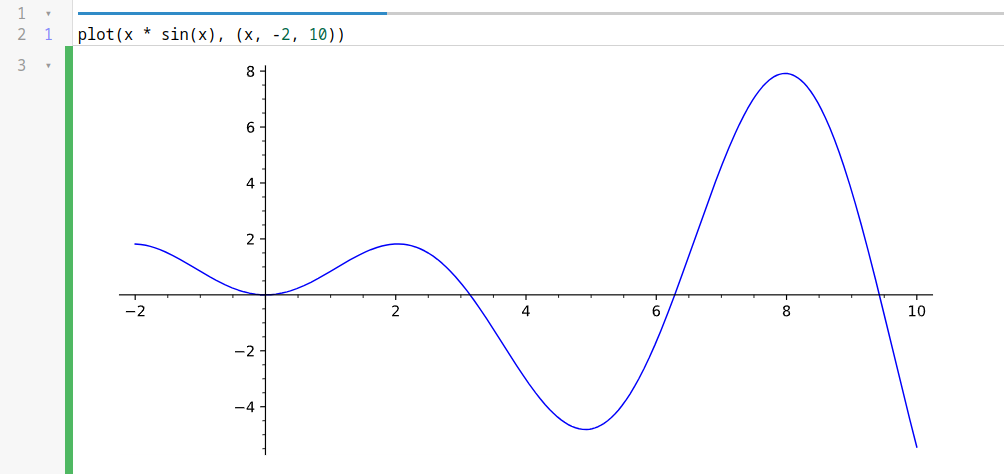
\includegraphics[scale=.4]{first_plot_screenshot.png}

\item Even more help is accessible from the top menu entry that's labelled, uhmmm, ``Help.''  There you can access the sage documentation, submit a support ticket if you think you've found a bug, or even have a chat with ChatGPT.  Try it!

\item When executing a cell produces an error message you can even ask for ``Artificial Intelligence help'' in correcting the problem.  It's possible to hold a back-and-forth conversation with ChatGPT that feels almost like talking to a human!

\item Some of you have probably already studied Calculus.  For others it will be coming up soon! The two main operations in Calculus (which are in a certain sense inverses of one another) are known as integration and differentiation.  Try using tab-completion and the help facility to find out how to do these operations in Sage.  It's pretty likely that you'll do something incorrect and get an error message.  If that happens try the ``Ask ChatGPT'' option.  Turn it into a conversation where you go back and forth with the AI a few times!

\end{enumerate}
